% ============================================================
%  Deliverable 3 slides: Results and Discussion
%  Build with:  pdflatex student-retention-results-slides.tex  (run twice for the outline)
%  Figures in figures/ are vector PDFs drawn from the executed analysis notebook
%  (student-retention-analytics.ipynb); the tables in figures/table_*.tex are generated from it.
% ============================================================
\documentclass[aspectratio=169,11pt]{beamer}
\usepackage[utf8]{inputenc}
\usepackage[T1]{fontenc}
\usepackage{lmodern}
\usepackage{amsmath}
\usepackage{amssymb}
\usepackage{booktabs}
\usepackage{graphicx}
\usepackage{microtype}
\usepackage{tikz}
\usepackage{tcolorbox}
\usetikzlibrary{arrows.meta,positioning}
\tcbuselibrary{skins}

% ---- colours shared with the whitepaper ----
\definecolor{paperblue}{RGB}{59,103,190}
\definecolor{titlebox}{RGB}{248,247,253}
\definecolor{good}{RGB}{30,132,73}
\definecolor{bad}{RGB}{192,57,43}
\definecolor{ink}{RGB}{35,40,52}
\definecolor{softgray}{RGB}{110,116,128}

% ---- theme: serif body, bold sans headings, no navigation clutter ----
\usetheme{default}
\usefonttheme{serif}
\setbeamertemplate{navigation symbols}{}
\setbeamercolor{normal text}{fg=ink}
\setbeamercolor{structure}{fg=paperblue}
\setbeamercolor{frametitle}{fg=paperblue}
\setbeamerfont{frametitle}{family=\sffamily\bfseries,size=\large}
\setbeamertemplate{frametitle}{%
  \vskip1.6mm\leavevmode\usebeamercolor[fg]{frametitle}\usebeamerfont{frametitle}\insertframetitle\par
  \vskip-1.0mm{\color{paperblue!35}\rule{\textwidth}{0.5pt}}}
\setbeamertemplate{itemize items}[circle]
\setbeamercolor{itemize item}{fg=paperblue}
\setbeamercolor{itemize subitem}{fg=paperblue}
\setbeamerfont{itemize/enumerate body}{size=\small}
\setbeamerfont{itemize/enumerate subbody}{size=\footnotesize}
\setlength{\leftmargini}{1.1em}
\setbeamersize{text margin left=0.9cm,text margin right=0.9cm}

\setbeamertemplate{footline}{%
  \leavevmode\hbox to\paperwidth{%
    \hspace{0.9cm}{\color{softgray}\sffamily\scriptsize Batitay \,$\cdot$\, Eskwelabs Fellowship \,$\cdot$\, Deliverable 3}%
    \hfill{\color{bad}\sffamily\bfseries\scriptsize SYNTHETIC DATA: not real students}%
    \hfill{\color{softgray}\sffamily\scriptsize\insertframenumber\,/\,\inserttotalframenumber}\hspace{0.9cm}}%
  \vskip3mm}

\newcommand{\key}[1]{\textcolor{paperblue}{\textbf{#1}}}
\newcommand{\fig}[2][\linewidth]{\centering\includegraphics[width=#1]{figures/#2}}
\newenvironment{figbul}{\begingroup\setbeamerfont{itemize/enumerate body}{size=\footnotesize}\begin{itemize}\setlength\itemsep{1.5pt}}{\end{itemize}\endgroup}

\hypersetup{pdftitle={Student Retention Analytics: Results and Discussion (Deliverable 3 slides)},pdfauthor={Matthew C. Batitay},pdfsubject={Eskwelabs Innovation Fellowship, Data Innovation Track},colorlinks=true,linkcolor=paperblue,urlcolor=paperblue}

\title{Student Retention Analytics: Results and Discussion}
\author{Matthew C. Batitay}

\begin{document}

% ------------------------------------------------------------ 1 title
\begin{frame}[plain]
\vspace{0.4cm}
\begin{tcolorbox}[colback=titlebox,colframe=titlebox,arc=4mm,boxrule=0pt,left=10mm,right=10mm,top=7mm,bottom=7mm]
\begin{center}
{\sffamily\bfseries\LARGE Does the Early-Warning System Work?\\[3pt] Prediction, Causation and Targeting in a Synthetic Student-Retention Cohort}\\[12pt]
{\large Matthew C. Batitay}\\[2pt]
{\itshape Eskwelabs Innovation Fellowship, Data Innovation Track}\\[8pt]
{\sffamily\small Deliverable 3: Results and Discussion}
\end{center}
\end{tcolorbox}
\vfill
\begin{center}
{\sffamily\bfseries\small\textcolor{bad}{Everything in this deck is synthetic.}}\\[2pt]
{\small Every number describes a generative model calibrated to cited aggregate statistics.\\ It is not a measurement of any real student, institution or programme.}
\end{center}
\vspace{0.3cm}
\end{frame}

% ------------------------------------------------------------ 2 setup
\begin{frame}{I use the data like an analyst, and the hidden truth only to grade my work}
\begin{columns}[T]
\column{0.5\textwidth}
\textbf{\sffamily The setup}
\begin{figbul}
\item A synthetic cohort of \key{50,000 students} over 8 terms, calibrated to cited Philippine attrition: \key{67.1\%} (high tier) and \key{45.9\%} (typical tier).
\item A \key{hidden} state (baseline vulnerability, acute shocks) drives the records \emph{and} the dropouts. An analyst sees only eight exported tables.
\item Support is assigned from prior-term signals, so it is \key{confounded}. The true effect is known: the dropout hazard is cut by \key{30\%}.
\end{figbul}
\column{0.5\textwidth}
\textbf{\sffamily The rules I held myself to}
\begin{figbul}
\item Analysis reads the \key{exported CSVs only}. The hidden truth is used in three labelled places, always to \emph{grade} the result.
\item \key{No leakage}: a feature for term $t$ uses entry attributes and terms $1$ to $t{-}1$ only.
\item Validation \key{grouped by student}; same folds for every model; nothing tuned on test data.
\item Every added choice tagged \texttt{LOCKED}, \texttt{CALIBRATED} or \texttt{ASSUMED}.
\end{figbul}
\end{columns}
\vfill
\begin{tcolorbox}[colback=titlebox,colframe=paperblue!40,boxrule=0.5pt,arc=2mm,left=3mm,right=3mm,top=2mm,bottom=2mm]
\small Because I know the answer, I can say whether each method gets the \emph{right} answer, not just whether it produces one.
\end{tcolorbox}
\end{frame}

% ------------------------------------------------------------ 3 six questions
\begin{frame}{Six questions, one chain of evidence}
\tikzset{q/.style={draw=paperblue!50,fill=titlebox,rounded corners=3pt,text width=4.2cm,minimum height=2.35cm,inner sep=5pt,align=left,font=\small}}
\centering
\begin{tikzpicture}
\node[q] at (0,0)    {{\sffamily\bfseries\textcolor{paperblue}{1. Is the generator valid?}}\\[2pt] 7 of 7 re-derived checks match the scorecard. The engine reproduces all 8 tables bit for bit.};
\node[q] at (4.65,0)  {{\sffamily\bfseries\textcolor{paperblue}{2. What does the data show?}}\\[2pt] Attrition 67.1\% vs 45.9\% by tier, highest for low-income working students.};
\node[q] at (9.3,0)  {{\sffamily\bfseries\textcolor{paperblue}{3. Can I predict dropout?}}\\[2pt] AUC \textbf{0.655} vs 0.567 for today's rule. Ceiling with perfect knowledge: 0.722.};
\node[q] at (0,-2.65)   {{\sffamily\bfseries\textcolor{paperblue}{4. Does support work?}}\\[2pt] The raw data say it \textbf{harms} ($-58\%$). Done right: \textbf{+32\%} against a true 30\%.};
\node[q] at (4.65,-2.65) {{\sffamily\bfseries\textcolor{paperblue}{5. Who is missed?}}\\[2pt] \textbf{64\%} of dropouts occur with a clean record and no support.};
\node[q] at (9.3,-2.65) {{\sffamily\bfseries\textcolor{paperblue}{6. How robust is this?}}\\[2pt] Holds across 11 recalibrated scenarios. IPW fails without overlap.};
\end{tikzpicture}
\end{frame}

% ------------------------------------------------------------ 4 validity
\begin{frame}{The generator holds up when I re-derive its checks from the CSVs}
\footnotesize
\centering
\begin{tabular}{@{}p{4.6cm}p{6.9cm}c@{}}
\toprule
Check & Re-derived from the exported tables & Result \\ \midrule
Tier attrition (calibrated) & High 67.1\%, typical 45.9\% (targets 67.1\%, 45.9\%) & pass \\
Correlation structure & Signals correlate ($+0.39$, $-0.19$, $-0.18$), but $\le 0.009$ once the hidden state is removed & pass \\
Confounding present & Naive estimate $-57.7\%$ (95\% CI $-64.6$ to $-50.6$) excludes the true 30\% & pass \\
Effect recoverable & Mantel--Haenszel 32.2\% (24.3 to 39.3); Poisson 33.6\% (25.1 to 41.2) & pass \\
Edge cases from the mechanism & 2,937 unflagged shock-driven dropouts; 774 falsely flagged terms & pass \\
Engine copy is faithful & All 8 tables regenerate with matching SHA-256; calibration loop returns the recorded values & pass \\ \bottomrule
\end{tabular}
\vspace{1mm}

\begin{tcolorbox}[colback=titlebox,colframe=paperblue!40,boxrule=0.5pt,arc=2mm,left=3mm,right=3mm,top=2mm,bottom=2mm]
\scriptsize \textbf{What this does not show.} It does not show the generator resembles any real institution. Calibration to the two tier targets is a convergence check, not independent validation. I did not re-run the generator's held-out Class-of-2023 check, which it labels \emph{pass (fragile)}.
\end{tcolorbox}
\end{frame}

% ------------------------------------------------------------ 5 descriptive
\begin{frame}{What the data shows: two tiers, a steep gradient, and a selection effect}
\fig{s1_descriptive.pdf}
\vspace{1mm}
\begin{figbul}
\item Per-term dropout \emph{falls} over time (high tier 15.4\% to 12.1\%): that is \key{selection}, since the most vulnerable leave first. It is not evidence that retention gets easier.
\item Attrition runs from about \key{35\%} (non-working, top income bracket) to \key{67\%} (working, lowest). The gradient is built into the generator: a structure check, not a finding about the world.
\end{figbul}
\end{frame}

% ------------------------------------------------------------ 6 prediction
\begin{frame}{Early warning works, but only modestly}
\fig{s2_prediction.pdf}
\vspace{1mm}
\begin{figbul}
\item \key{Boosted trees: AUC 0.655} (fold SD 0.005) against 0.567 for the signal-count rule. A logistic hazard gets 0.654, so the signal is nearly additive.
\item Reviewing the top \key{10\%} of student-terms captures \key{21.4\%} of dropouts (rule: 15.3\%); calibration is good in every decile.
\item Drivers: the \emph{running averages} of prior grades and attendance, not last term's flags.
\end{figbul}
\end{frame}

% ------------------------------------------------------------ 7 ceilings
\begin{frame}{How good could any model be? The hidden truth sets the ceiling}
\centering\footnotesize
\setlength{\tabcolsep}{5pt}\begin{tabular}{@{}lccccc@{}}\toprule
Model & AUC & PR-AUC & Top 5\% & Top 10\% & Top 20\% \\
\midrule
Signal-count rule & 0.567 & 0.104 & 8.2\% & 15.3\% & 29.9\% \\
Logistic hazard & 0.654 & 0.139 & 12.1\% & 21.1\% & 36.7\% \\
Boosted trees & 0.655 & 0.140 & 12.2\% & 21.4\% & 36.9\% \\
\midrule
\textit{Leaky: + current-term signals (not deployable)} & 0.680 & 0.163 & 14.6\% & 24.8\% & 40.4\% \\
\textit{Ceiling B: knows baseline vulnerability} & 0.683 & 0.159 & 13.9\% & 24.2\% & 40.8\% \\
\textit{Ceiling A: true hazard} & 0.722 & 0.219 & 19.7\% & 31.1\% & 47.4\% \\
\bottomrule
\end{tabular}
\\[1mm]
{\scriptsize Out-of-fold, 247,739 student-terms (terms 2 to 8), event rate 8.0\%. ``Top $x$\%'' = share of dropouts captured by reviewing the top $x$\% of student-terms.}
\vspace{1.5mm}

\begin{columns}[T]
\column{0.32\textwidth}
\begin{tcolorbox}[colback=titlebox,colframe=paperblue!40,boxrule=0.5pt,arc=2mm,left=2mm,right=2mm,top=1.5mm,bottom=1.5mm]
\footnotesize \textbf{Much of dropout cannot be foreseen.} Even the true hazard gives AUC 0.722, because this term's shock is unknowable in advance.
\end{tcolorbox}
\column{0.32\textwidth}
\begin{tcolorbox}[colback=titlebox,colframe=paperblue!40,boxrule=0.5pt,arc=2mm,left=2mm,right=2mm,top=1.5mm,bottom=1.5mm]
\footnotesize \textbf{19.4\% of dropouts} (4,762 of 24,573) happen in term 1, before any record exists. No term-based model can see them.
\end{tcolorbox}
\column{0.32\textwidth}
\begin{tcolorbox}[colback=titlebox,colframe=paperblue!40,boxrule=0.5pt,arc=2mm,left=2mm,right=2mm,top=1.5mm,bottom=1.5mm]
\footnotesize \textbf{Leaving out regional tier costs nothing} (AUC 0.655 vs 0.656), so excluding it on ethical grounds has no accuracy price here.
\end{tcolorbox}
\end{columns}
\end{frame}

% ------------------------------------------------------------ 8 actionability gap
\begin{frame}{A good predictor cannot tell me whether support works}
\begin{columns}[c]
\column{0.58\textwidth}
\fig[\linewidth]{s3_gap.pdf}
\column{0.42\textwidth}
\begin{itemize}\setlength\itemsep{4pt}
\item \textcolor{bad}{\textbf{Raw comparison: $-58\%$.}} Support goes to the students most at risk, so it looks harmful (confounding by indication).
\item \textcolor{orange!85!black}{\textbf{Stratify on the model's score: $+7\%$}} (CI $+3.0$ to $+11.7$). Right sign, but it misses the truth.
\item \textcolor{good}{\textbf{Stratify on the assignment signals: $+32.2\%$}} (CI $+24.3$ to $+39.3$). Covers the true 30\%.
\end{itemize}
\vspace{1mm}
\small Ranking students and evaluating a programme need \key{different designs}.
\end{columns}
\end{frame}

% ------------------------------------------------------------ 9 DAG
\begin{frame}{Why: a hidden common cause opens a backdoor path}
\centering
\resizebox{0.93\linewidth}{!}{%
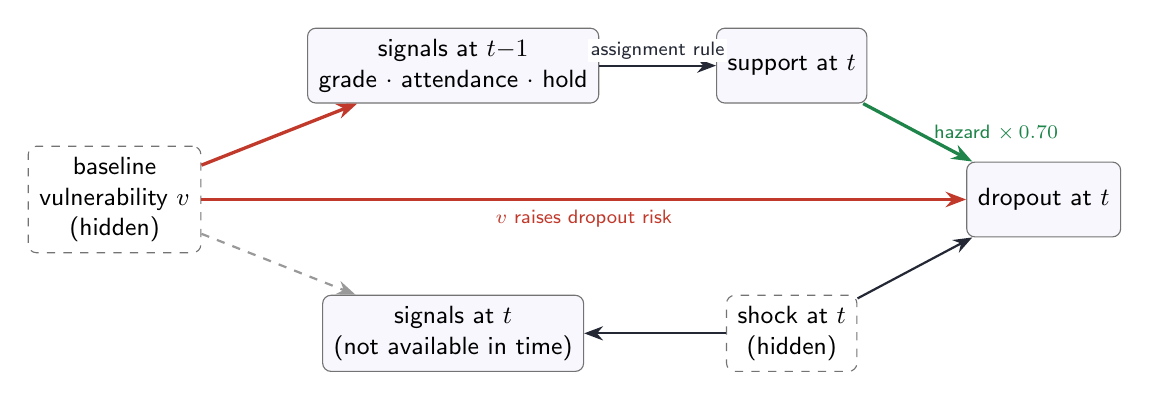
\begin{tikzpicture}[
  obs/.style={draw=black!55,rounded corners=3pt,fill=titlebox,minimum height=0.95cm,align=center,font=\sffamily\small,inner sep=4pt},
  lat/.style={obs,dashed,fill=white},
  arr/.style={-{Stealth[length=2.4mm]},thick,ink},
  red/.style={-{Stealth[length=2.6mm]},very thick,bad},
  grn/.style={-{Stealth[length=2.6mm]},very thick,good}]
\node[lat] (v)  at (0,0)     {baseline\\vulnerability $v$\\(hidden)};
\node[obs] (o1) at (4.3,1.7) {signals at $t{-}1$\\grade $\cdot$ attendance $\cdot$ hold};
\node[obs] (T)  at (8.6,1.7) {support at $t$};
\node[obs] (D)  at (11.8,0)  {dropout at $t$};
\node[lat] (S)  at (8.6,-1.7) {shock at $t$\\(hidden)};
\node[obs] (o2) at (4.3,-1.7) {signals at $t$\\(not available in time)};
\draw[red] (v) -- (o1);
\draw[red] (v) -- node[below,font=\sffamily\scriptsize,text=bad]{$v$ raises dropout risk} (D);
\draw[arr] (o1) -- node[above,yshift=1pt,font=\sffamily\scriptsize,fill=white,inner sep=1pt]{assignment rule} (T);
\draw[grn] (T) -- node[right,xshift=2pt,font=\sffamily\scriptsize,text=good]{hazard $\times\,0.70$} (D);
\draw[arr] (S) -- (D);
\draw[arr] (S) -- (o2);
\draw[arr,black!40,dashed] (v) -- (o2);
\end{tikzpicture}}
\vspace{1mm}
\begin{itemize}\setlength\itemsep{2pt}
\item The path \textcolor{bad}{support $\leftarrow$ signals$(t{-}1)$ $\leftarrow v \rightarrow$ dropout} is open, which is why the raw comparison fails.
\item Support depends \emph{only} on the signals at $t{-}1$, so within a signal cell it is as good as random: \key{stratify on those signals}.
\item The shock at $t$ is independent of everything before it, so it cannot confound.
\end{itemize}
\end{frame}

% ------------------------------------------------------------ 10 estimators
\begin{frame}{Estimator choice matters more than sample size}
\fig{s4_estimators.pdf}
\vspace{1mm}
\begin{figbul}
\item \key{Mantel--Haenszel and Poisson} recover about 30\% (SD about 4 points over 20 populations): one study resolves the effect to roughly $\pm 8$ points.
\item \textcolor{bad}{\textbf{IPW swings from $-47\%$ to $+72\%$}} over the same populations: the supported arm's \emph{effective} sample size is \textbf{43} of 15,293 (and I gave IPW the true propensity).
\end{figbul}
\end{frame}

% ------------------------------------------------------------ 11 adjustment sets
\begin{frame}{Adjusting for only some of the referral signals fails}
\fig{s5_adjustment.pdf}
\vspace{1mm}
\begin{figbul}
\item Grade only $-7.0\%$, attendance only $-20.4\%$, hold only $-37.1\%$. \key{Only the full set (+32.2\%) or the count of signals (+32.4\%) recovers the effect.}
\item \key{Log the inputs to the referral decision, not just the flag}, or the programme looks harmful however well it works. Only six cells hold both arms, so effect heterogeneity is out of reach.
\end{figbul}
\end{frame}

% ------------------------------------------------------------ 12 targeting
\begin{frame}{Most dropouts happen where the programme is not looking}
\fig{s6_targeting.pdf}
\vspace{1mm}
\begin{figbul}
\item \key{63.7\%} of dropout events fall in clean-record, unsupported terms; only 9.4\% fall in supported terms (6.2\% of all terms).
\item At equal capacity (15,293 slots) the model ranking averts an expected \key{940} dropouts against \key{796} for the actual rule (+18\%), but only 66\% of an unattainable oracle (1,421). This assumes a homogeneous 30\% effect.
\end{figbul}
\end{frame}

% ------------------------------------------------------------ 13 robustness
\begin{frame}{The conclusions survive what I varied}
\begin{columns}[c]
\column{0.5\textwidth}
\fig[\linewidth]{s7_sensitivity.pdf}
\column{0.5\textwidth}
\begin{figbul}
\item \key{11 scenarios}, each re-fitted to the same 67.1\% / 45.9\% targets, so differences are not just differences in attrition level.
\item \key{Mantel--Haenszel stays near 30\%} everywhere (replicate means 26.9\% to 30.1\%).
\item \textcolor{bad}{\textbf{IPW instability is a positivity problem}}: its SD falls from 35.6 points (default rule) to 1.1 (softest rule) as every signal cell gains both arms.
\item Predictability is \key{capped by baseline vulnerability}: ceiling B stays within 0.659 to 0.686, while ceiling A ranges from 0.696 to 0.800 with shock strength.
\end{figbul}
\end{columns}
\end{frame}

% ------------------------------------------------------------ 14 recommendations
\begin{frame}{Recommendations: how to build and evaluate a retention programme}
\begin{columns}[T]
\column{0.5\textwidth}
\begin{enumerate}\setlength\itemsep{2.5pt}\small
\item \key{Triage, do not judge.} Use the risk model to allocate attention, never to evaluate the programme.
\item \key{Evaluate with the assignment rule.} Log the referral inputs with the support flag; use Mantel--Haenszel or clustered Poisson. Expect $\pm 8$ points at 50,000 students.
\item \key{Build overlap into the rollout.} A small randomised share of referrals makes IPW and cell estimates usable.
\item \key{Pilot model-based allocation} head to head with the current rule before trusting the +18\%.
\end{enumerate}
\column{0.5\textwidth}
\begin{enumerate}\setlength\itemsep{2.5pt}\small\setcounter{enumi}{4}
\item \key{Look where the dropouts are,} not only where the flags are (64\% have a clean record).
\item \key{Keep regional tier out} of the flagging model (no accuracy cost here).
\item \key{Handle IPW with care} under steep assignment: report effective sample size and largest weights.
\item \key{Do not act on these numbers.} The method is the point: validate against known truth, separate prediction from causation, and test how much each conclusion depends on assumptions.
\end{enumerate}
\end{columns}
\end{frame}

% ------------------------------------------------------------ 15 limitations
\begin{frame}{What these results are not}
\begin{itemize}\setlength\itemsep{2.5pt}
\item \key{Everything is a property of the generator.} The prediction ceilings, the homogeneous 30\% effect and the form of the confounding are assumptions, not measurements.
\item \key{The causal problem here is easier than a real one.} Support never changes later grades (no carry-over), assignment has no unobserved drivers or caseworker discretion, the analyst knows the thresholds, and IPW gets the true propensity.
\item \key{The targeting gain is conditional.} The policy value assumes the same 30\% effect for everyone, so ranking by risk is optimal by construction.
\item \key{The model comparison is narrow.} Two model families, fixed hyperparameters, one population; the sensitivity grid varies one parameter at a time with 10 replicates each.
\item \key{Open items.} The generator's held-out check is fragile and was not re-run; the mechanism behind the biased score-stratified estimate is not investigated; term-1 dropouts (19.4\%) fall outside both analyses.
\end{itemize}
\vspace{1mm}
{\scriptsize Full list with status: notebook Section 12 (flags OF-1 to OF-12 from the generator, DF-1 to DF-9 new here).}
\end{frame}

% ------------------------------------------------------------ 16 takeaways
\begin{frame}{Take-aways}
\begin{tcolorbox}[colback=titlebox,colframe=paperblue!40,boxrule=0.5pt,arc=2mm,left=4mm,right=4mm,top=3mm,bottom=3mm]
\begin{enumerate}\setlength\itemsep{5pt}
\item A risk model \key{ranks} students. It does not tell me whether the support \key{works}.
\item Evaluating support needs the \key{assignment inputs}, the right adjustment set, and \key{overlap} between those who were and were not supported.
\item Inside this synthetic world a better ranking buys \key{modestly} more, because much of dropout is unforeseeable and most of it happens where no flag is raised.
\end{enumerate}
\end{tcolorbox}
\vspace{2mm}
\small
\textbf{\sffamily Where to find it.} Notebook: \texttt{results-and-discussion/student-retention-analytics.ipynb} (executed copy: \texttt{.html}). It runs end to end from the exported CSVs, and every output carries a synthetic-data banner. Dataset and generator: \texttt{synthetic-data-generator/}. Specification: whitepaper v17.
\end{frame}

% ------------------------------------------------------------ 17 references
\begin{frame}{References}
\footnotesize
\setlength{\parindent}{0pt}\setlength{\parskip}{4pt}
Gelman, A., Hill, J., and Vehtari, A. (2020). \emph{Regression and Other Stories}. Cambridge University Press, Cambridge, U.K.

James, G., Witten, D., Hastie, T., and Tibshirani, R. (2013). \emph{An Introduction to Statistical Learning with Applications in R}. Springer, New York, NY.

Law, A. M. (2015). \emph{Simulation Modeling and Analysis}, 5th edition. McGraw-Hill, New York, NY.

Lopez-Mu\~noz, G. L., Gonzalez Serrano, C., and Sanchez-Ferreira, C. (2026). Student Dropout Prediction in Higher Education: A Systematic Review of Machine Learning Methods and Risk Factors. \emph{Journal of Information Technology Education: Research}, 25, Article 20. \url{https://doi.org/10.28945/5776}

Peters, J., Janzing, D., and Sch\"olkopf, B. (2017). \emph{Elements of Causal Inference: Foundations and Learning Algorithms}. MIT Press, Cambridge, MA.

\vspace{2mm}
{\scriptsize The generator's calibration sources (CPBRD 2025; EDCOM II 2025; CHED 2025) are traced in the whitepaper, Section 10.}
\end{frame}

% ============================================================ backup
\appendix
\begin{frame}{Backup A: policy values at equal capacity}
\centering\footnotesize
\setlength{\tabcolsep}{5pt}\begin{tabular}{@{}lrrrr@{}}\toprule
Policy (15,293 slots) & Averted & Per 100 slots & \% of oracle & Slots per averted \\
\midrule
Actual programme & 796 & 5.20 & 56.0\% & 19.2 \\
Boosted-tree ranking & 940 & 6.15 & 66.2\% & 16.3 \\
Signal-count rule, ties at random & 809 & 5.29 & 56.9\% & 18.9 \\
Oracle (true untreated hazard) & 1,421 & 9.29 & 100.0\% & 10.8 \\
Random & 375 & 2.45 & 26.4\% & 40.8 \\
\bottomrule
\end{tabular}
\\[2mm]
{\footnotesize Expected values inside the model: a slot is worth $0.30\times$ the student-term's untreated hazard. Capacity is the number of supported student-terms in terms 2 to 8 (6.2\% of 247,739). Total avertable if every term were supported: 6,097 dropouts.}
\vspace{3mm}

\begin{itemize}\small\setlength\itemsep{2pt}
\item The oracle ranks by true untreated hazard, which includes \emph{this term's shock}. That is why it is unattainable, and why a below-average-vulnerability student can still be its best pick.
\item The signal-count rule with random ties performs like the actual rule, since the actual rule is that rule plus noise.
\end{itemize}
\end{frame}

\begin{frame}{Backup B: sensitivity grid in numbers}
\centering\scriptsize
\setlength{\tabcolsep}{3.5pt}\begin{tabular}{@{}lrrrrrrr@{}}\toprule
Scenario & Supp. & Naive & MH & MH SD & IPW SD & AUC rule & AUC B/A \\
\midrule
Baseline $(-9,6)$ & 6.2\% & $-$57.7\% & +32.2\% & 5.0 & 35.6 & 0.565 & 0.683/0.722 \\
$\beta_0{=}-7,\beta{=}6$ & 10.7\% & $-$38.0\% & +33.5\% & 1.5 & 19.5 & 0.558 & 0.680/0.720 \\
$\beta_0{=}-5,\beta{=}3$ & 7.0\% & $-$35.3\% & +33.8\% & 2.6 & 5.6 & 0.566 & 0.684/0.723 \\
$\beta_0{=}-3,\beta{=}2$ & 12.9\% & $-$10.3\% & +33.1\% & 1.5 & 2.3 & 0.563 & 0.683/0.723 \\
$\beta_0{=}-2,\beta{=}1$ & 17.0\% & +12.1\% & +32.3\% & 1.0 & 1.1 & 0.570 & 0.686/0.726 \\
Shock prob.\ 0.04 & 5.6\% & $-$59.0\% & +30.9\% & 5.0 & 36.7 & 0.564 & 0.684/0.707 \\
Shock prob.\ 0.16 & 7.4\% & $-$52.5\% & +31.8\% & 4.6 & 39.4 & 0.562 & 0.679/0.743 \\
$\gamma_2{=}0.75$ & 6.3\% & $-$58.3\% & +31.0\% & 5.6 & 37.4 & 0.565 & 0.686/0.696 \\
$\gamma_2{=}3.0$ & 6.1\% & $-$49.8\% & +35.0\% & 5.2 & 51.3 & 0.556 & 0.659/0.800 \\
Grade noise 4 & 4.9\% & $-$74.9\% & +32.2\% & 4.2 & 37.5 & 0.561 & 0.684/0.722 \\
Grade noise 16 & 8.2\% & $-$37.7\% & +30.9\% & 3.6 & 38.9 & 0.557 & 0.682/0.722 \\
\bottomrule
\end{tabular}
\\[2mm]
{\tiny Each scenario recalibrated to 67.1\% / 45.9\%. Estimates are relative reductions (truth $+30\%$). ``MH SD'' and ``IPW SD'' are SDs in percentage points over 10 replicate populations. ``Supp.'' is the share of student-terms (terms 2 to 8) that receive support.}
\end{frame}

\end{document}
